The multi-model concept was introduced in \mf using GWF Model Exchange objects to support a tight coupling between any two groundwater flow models at the matrix level. This concept turned out rather successful and valued by the modeling community, but the implementation had its drawbacks too. The information on the spatial discretization at the interface as it is available in the Model Exchange object is limited, designed to carry out the basic conductance calculation between connected cells. For example, the XT3D option in the NPF package enables simulation of fully three-dimensional (3D) anisotropy taking into account the full, three-dimensional conductivity tensor \cite{modflow6xt3d}. In doing so it requires geometrical data, not only from the two connected cells but also from their neighbors. These data are not available in the Model Exchange object and the XT3D option could not be applied across the model interface, at least not without a significant restructuring of the code. The enhancement of \mf with the transport model (GWT) \cite{???} has illustrated the need for a more generic coupling of sub-models too. Here the XT3D option is used in a similar fashion for the dispersion calculation and the TVD (total variation diminishing) scheme in the advective transport calculation has a computational stencil that requires information from neighboring cells as well. Finally, the GWF Model Exchange object merely replicates logic that was already present in the standard GWF packages, e.g. the standard NPF conductance calculation and the cell rewetting algorithm, and is not easily extended with additions to those packages. To address these challenges and extend \mf with the capability to couple GWT models, the concept of an Interface Model has been introduced.

\subsection{Interface Model}

- coefficient provider, identical to how exchange does that
- interface model is basis for computation: it is just a GWF or GWT model potentially all features
- puts conditions on relative position models (topological sanity)
- describe how the grid is created
- maybe also how and which packages are added?

\begin{figure}[!ht]
	\begin{center}
	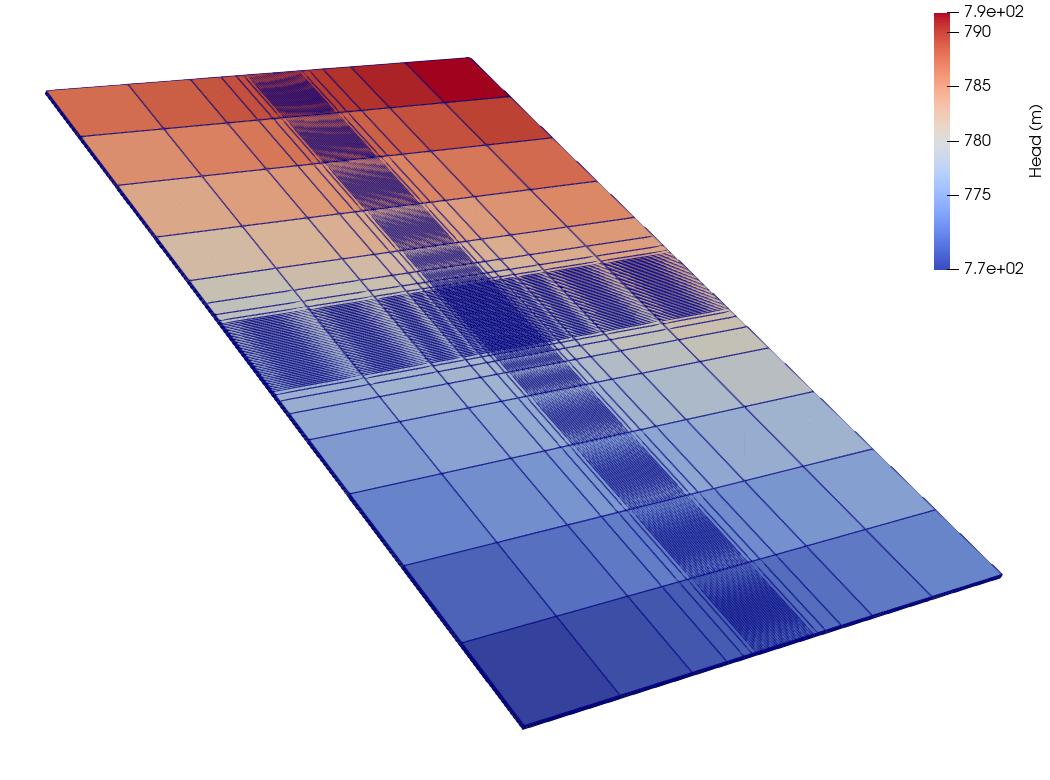
\includegraphics[scale=0.35]{./Figures/InterfaceModel/gwt-ifmod-full.png}
	\caption[The full model grid from MT3DMS problem 10]{The full model grid for the simulation as described in MT3DMS problem 10 as a composition of two GWF submodels with a GWF-GWF exchange, and two GWT submodels with a GWT-GWT exchange.}
	\label{fig:gwtgwt-fullgrid}
	\end{center}
\end{figure}

\begin{figure}[!ht]
	\begin{center}
	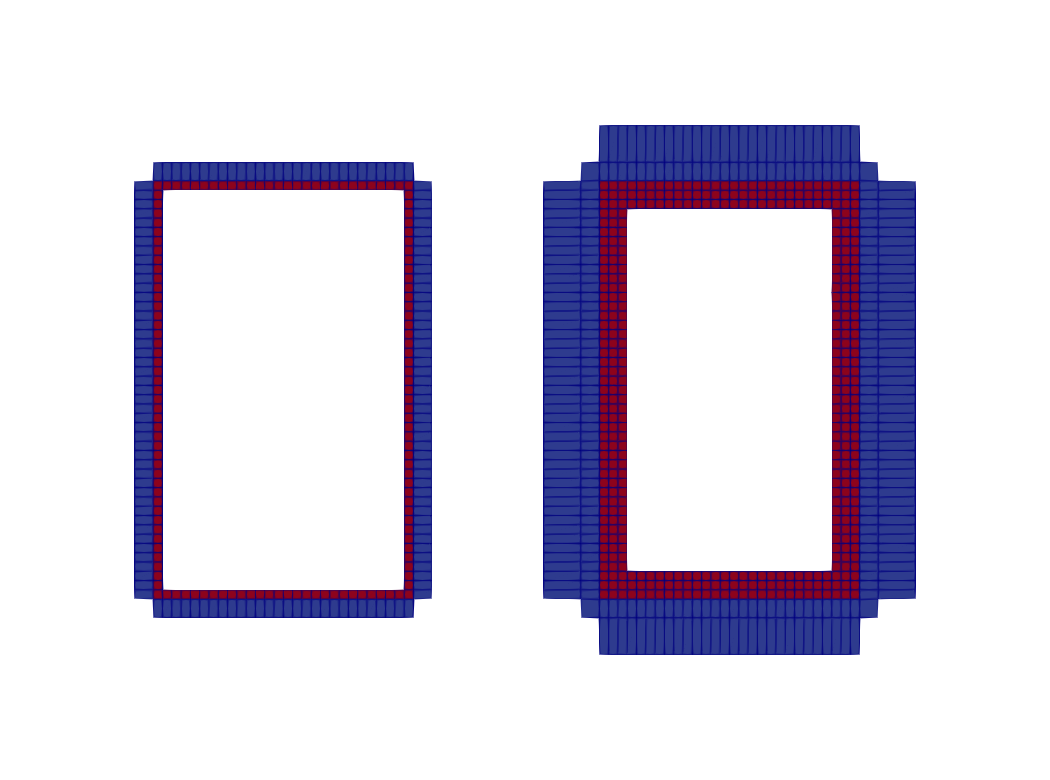
\includegraphics[scale=0.5]{./Figures/InterfaceModel/gwt-ifmod-ifgrids.png}
	\caption[The GWF and the GWT interface grid for the inner model]{The GWF and the GWT interface grid for the inner model.}
	\label{fig:gwtgwt-fullgrid}
	\end{center}
\end{figure}

\begin{figure}[!ht]
	\begin{center}
	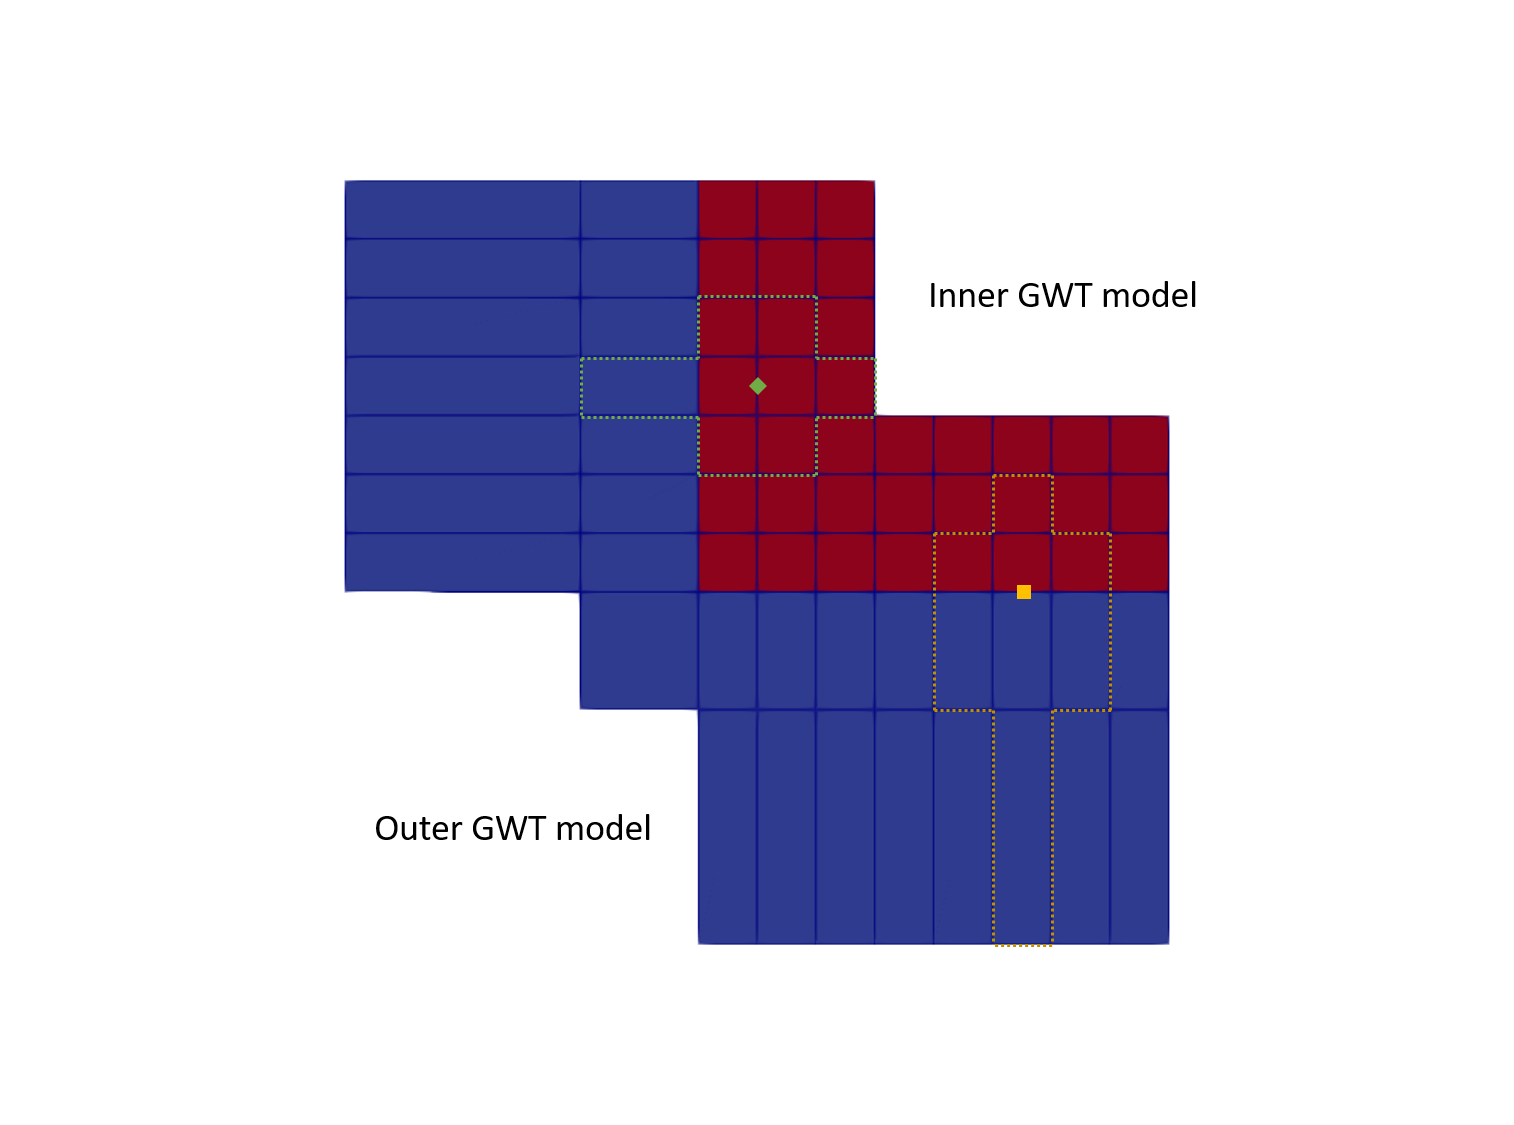
\includegraphics[scale=0.5]{./Figures/InterfaceModel/gwt-ifmod-stencils.png}
	\caption[The stencils]{The stencils.}
	\label{fig:gwtgwt-fullgrid}
	\end{center}
\end{figure}